\section{研究内容与技术路线}

本课题拟实现一个基于法条的判案论点细粒度挖掘的司法辅助系统,
本论文的工作分为如下几个方面,如\cref{fig_1}所示。
该系统首先细粒度解耦法律条文,
根据法律条文获得分析案件所需的维度。
在此基础上,以案情描述作为输入,基于细粒度解耦的法律条文,
自动挖掘判案论点并且自动识别案情描述中的关键信息。
最后,根据判案论点和案情描述中的关键信息,
分析论证每一个判案论点所需的证据,
预测该案件判决为某罪名所需的完备证据集。
上述三个功能组合成完整的司法辅助系统,
从而能够辅助司法从业者分析理解与决策。
\begin{figure}[h]
	\centering
	% 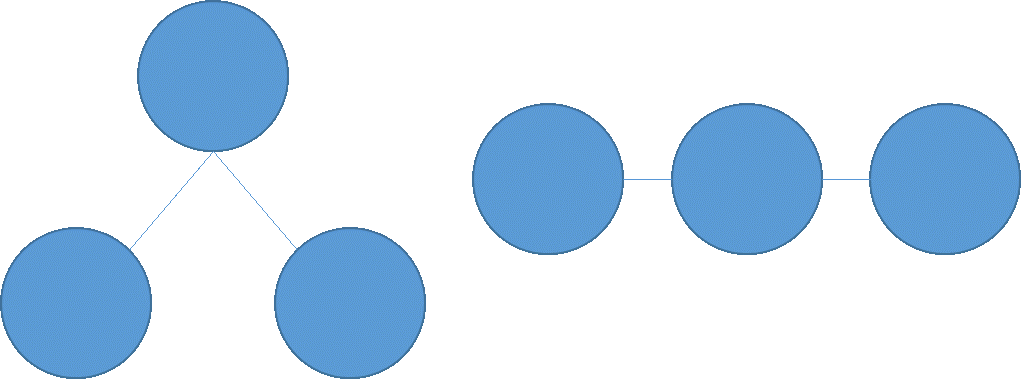
\includegraphics[width=0.4\linewidth]{fig_1.png}

	\scriptsize
	\tikzstyle{format}=[rectangle,draw,fill=white,font=\fontsize{12pt}{18pt}\selectfont]
	\begin{tikzpicture}
		\node[format] (law){法律条文细粒度解耦};
		\node[format,right of=law,node distance=45mm] (argument){判案论点挖掘};
		\node[format,right of=argument,node distance=45mm] (key_info){案情描述关键信息识别};
		\node[format,below of=argument,node distance=15mm] (evidence){完备证据集预测};
		\node[format,below of=key_info,node distance=15mm] (legal){司法下游任务};
		\draw[->] (law)--(argument);
		\draw[->] (argument)--(key_info);
		\draw[->] (argument)--(evidence);
		\draw[->] (key_info)--(evidence);
		\draw[->] (key_info)--(legal);
		% \draw[->](setkeycheck)--node[above]{Yes}(setsetflag);
		% \draw[->](setkeycheck) --node[left]{No} (readtime);
	\end{tikzpicture}
	\caption{研究内容关系示意图}
	\label{fig_1}
\end{figure}

\subsection{研究内容一:法律条文细粒度解耦}
根据现有的司法法律条文,我们从法律条文中细粒度解耦出分析案件所需的维度。
法律条文的内容具有一定的抽象性、概括性、精确性和整体性。
从学理上将,中国是典型的大陆法系国家,
大陆法系要求法官遵从法律明文办理案件,
这与英美法系的判例法有着明显的区别。
所以,辅助国内司法从业者,
就需要对法条进行细粒度解耦,
并根据解耦的要素来指导进一步对案情描述的分析。

\subsection{研究内容二:判案论点挖掘}
对于一篇给定的案情描述,
我们拟基于法律条文解耦得到的重要维度,
自动总结出该案件的判案论点。
之后,根据每一个判案论点,
从案情描述中自动识别出对应关键信息,
将法律条文与案情描述进行论点上的关联和维度上的对应。
这一部分的判案论点和关键信息可以被使用于罪名预测、法条预测等司法下游任务,
该种方式不仅具有更强的可解释性,
而且能够更好的辅助司法从业人员理解案情、书写文书以及做出决策。

\subsection{研究内容三:司法证据集预测与生成}
在司法案件中,完备的证据集至关重要,
其在定罪与量刑中起着决定性的作用。
所以根据一个案件的案情描述,总结出其完备的证据集,
能够很好的辅助到司法从业者。
我们拟基于案情描述的文本信息以及上述挖掘的判案论点,
根据每一个论点预测生成对应证据,
列举完备的论据可以充分论证判案论点,
从而构建出完备的证据集。

\subsection{XXXXX方法技术路线}

本文使用XXX方法技术路线,如\cref{fig_2}所示。

\begin{figure}[h]
	\centering
	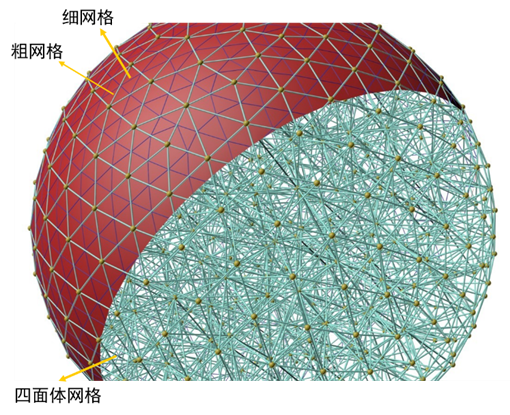
\includegraphics[width=0.6\linewidth]{fig_2.png}
	\caption{本论文拟构建的物理仿真模型示意图}
	\label{fig_2}
\end{figure}

\subsection{XXXXX方法技术路线}

\subsection{XXXXX方法技术路线}